\section{Shape-Truthful Clustering (Shatter)}

\subsection{Overview of Multi-Dimensional, Multi-Variate Data}
When working with vectors in space, our goal is to cluster them according to different characteristics:
\begin{itemize}
    \item Density
    \item Cosine (conserved direction)
    \item Energy (norm of vectors in volume)
    \item More complex Clustering Characteristics (CC)
\end{itemize}

\begin{figure}[h!]
    \centering
    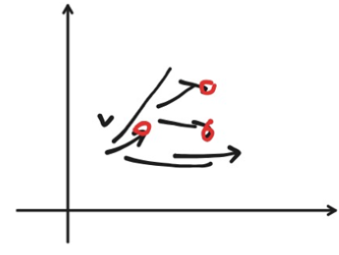
\includegraphics[width=0.5\textwidth]{figures/shatter_vectors_1a.png}
    \caption{Vectors in space, evaluated by complex clustering characteristics.}
    \label{fig:shatter_vectors}
\end{figure}

\subsection{Algorithm Sketch}
To illustrate the algorithm, we use \textbf{Local Density} as an example Clustering Characteristic (CC).

\begin{enumerate}
    \item \textbf{Construct Local Labeling Volume (LV):} Around each vector, construct a local sphere of fixed size (parameter $r$). Note that this volume can also be a cone around the direction the vector points to. We call this property the Local Labeling Volume (LV).
    \item \textbf{Assign Labels:} The LV collects neighboring vectors which are used to produce a real label for the vector. For example, density (the number of vectors in the LV) or angular variance (a measure of the agreement in direction of the vectors in the LV cone). All data vectors receive real labels.
    \item \textbf{Sort and Select:} Sort the data vectors descending by their labels. Start with the top quantile (parameter \texttt{label\_quantile}) of labels as seed nodes.
    \item \textbf{Graph Construction:} Using a K-D-Tree, create a graph where nodes are the data vectors and edges connect to \textit{direct} neighbors. We may need to use a neighbor radius. Direct neighbors can be defined by:
    \begin{itemize}
        \item Overlap of LVs
        \item Lying within each other's LV
        \item Being within a fixed radius
    \end{itemize}
\end{enumerate}

\begin{figure}[h!]
    \centering
    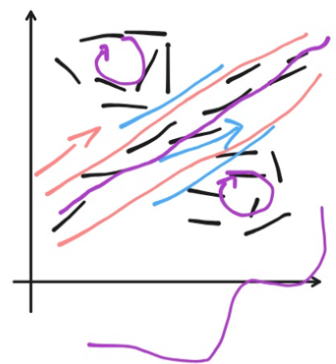
\includegraphics[width=0.6\textwidth]{figures/shatter_vectors_1b.png}
    \caption{Iterative cluster growth along defined local volumes.}
    \label{fig:shatter_clusters}
\end{figure}

\subsection{Iterative Cluster Growth}
To track the state of the graph, we maintain a list of visited edges and a list of nodes assigned to clusters.

\begin{enumerate}
    \item Select start nodes (e.g., the top quantile of labels).
    \item In parallel, grow clusters iteratively (one step/edge per iteration).
    \item Per iteration, add all unvisited edges reaching out from nodes already in the current cluster.
    \item Add nodes that do not reduce the mean CC dramatically, utilizing an error term (parameter $\tau$).
    \item \textbf{Merging:} If you reach nodes that are already in a different cluster, mark those two clusters as Potential Merge Candidates (PMC).
    \item \textbf{Stop Conditions:} Halt if all edges are visited, or all clusters have grown until the CC stop condition is met.
    \item \textbf{Experimental Exploration:} If nodes are not assigned to clusters yet, repeat the above process, starting with the upper quantile of labels from the nodes not yet assigned a cluster.
\end{enumerate}